\documentclass[a3paper,12pt]{extarticle} % Use extarticle for A3 paper size
\usepackage{graphicx} % Include this package for \includegraphics
\usepackage{amsmath}
\usepackage{amssymb} % Include this package for \mathbb
\usepackage[margin=1in]{geometry} % Adjust the margin as needed

\begin{document}

\author{kipngeno koech - bkoech}
\title{Homework 3 - Introduction to Machine Learning for Engineers}   
\maketitle

\medskip

\maketitle
\section{Dimensionality of K-Nearest Neighbors}

When the number of features $d$ is large, the performance of $k$-nearest neighbors, which makes predictions using only observations that are near the test observation, tends to degrade. This phenomenon is known as the \textit{curse of dimensionality}, and it ties into the fact that non-parametric approaches often perform poorly when $d$ is large.

\begin{enumerate}
    \item Suppose that we have a set of training observations, each corresponding to a one-dimensional ($d = 1$) feature, $X$. We assume that $X$ is uniformly (evenly) distributed on $[0, 1]$. Associated with each training observation is a response value.Suppose that we wish to predict a test observation $x$'s response using only training observations that are within $10\%$ of the range of $x$ closest to that test observation. In other words, if $x \in [0.05, 0.95]$ then we will use training observations in the range $[x - 0.05, x + 0.05]$, as shown in Figure 1 when $x = 0.6$. When $x \in [0, 0.05)$ we use the range $[0, 0.1]$, and when $x \in (0.95, 1]$ we use training observations in the range $[0.9, 1]$. Figure 1 shows this range for $x = 0.02$.On average (assuming $x$ is uniformly distributed on $[0, 1]$), what fraction of the available observations will we use to make the prediction?
    \item Now suppose that we have a set of observations, each corresponding to two features, $X_1$ and $X_2$ (i.e., $d = 2$). We assume that $(X_1, X_2)$ are uniformly distributed on $[0, 1] \times [0, 1]$. We wish to predict the response of a test observation $(x_1, x_2)$ using only training observations that are within $10\%$ of the range of $x_1$ and within $10\%$ of the range of $x_2$ closest to that test observation. For instance, in order to predict the response for a test observation with $x_1 = 0.6$ and $x_2 = 0.04$, we will use training observations $(X_1, X_2)$ such that $X_1 \in [0.55, 0.65]$ and $X_2 \in [0, 0.1]$.
    \begin{figure}[h]
        \centering
        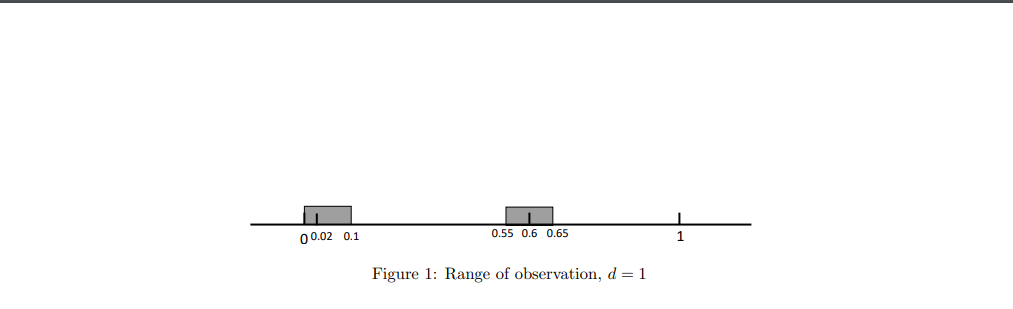
\includegraphics[width=0.8\textwidth]{section1.png}
        \caption{Primal Formulation of SVM}
        \label{fig:primal}
    \end{figure}
    \item On average, assuming $x_1$ and $x_2$ are each uniformly distributed on $[0, 1]$, what fraction of the available observations will we use to make the prediction?
    \item Now suppose that we have a set of training observations on $d = 100$ features. Again, the observations are uniformly distributed on each feature, and again each feature ranges in value from $0$ to $1$. We wish to predict a test observation’s response using observations within the $10\%$ of each feature’s range that is closest to that test observation. What fraction of the available observations will we use to make the prediction?
    \item Using your answers to parts a–c, argue that a drawback of $k$-nearest neighbors when $d$ is large is that there are very few training observations “near” any given test observation.
    \item Now suppose that we wish to make a prediction for a test observation by creating a $d$-dimensional hypercube centered around the test observation that contains, on average, $10\%$ of the training observations. For $d = 1$, $2$, and $100$, what is the length of each side of the hypercube? How does your answer change as $d$ increases, and what does this imply for the accuracy of $k$-nearest neighbors when $d$ is large?
    
    \textbf{Note:} A hypercube is a generalization of a cube to an arbitrary number of dimensions. When $d = 1$, a hypercube is simply a line segment; when $d = 2$, it is a square; and when $d = 100$, it is a $100$-dimensional cube.
\end{enumerate}
\newpage

\section{Decision Trees}


\end{document}